\documentclass{beamer}
\usepackage[english]{babel}
\usepackage{calc}
\usepackage[absolute,overlay]{textpos}
\usepackage{amsmath, amsthm, amssymb, enumerate}
\usepackage{mathtools}
\usepackage{blkarray}
\usepackage{tikz}
\usepackage{tikz-cd}
\usepackage{quiver}
\usepackage{graphicx}
\usepackage{xcolor}
\usepackage{standalone}
\usepackage{yhmath}
\usetikzlibrary{matrix,decorations.pathreplacing,calc,positioning}


\useoutertheme{split}
\setbeamertemplate{navigation symbols}{}

\newcommand{\unc}[1]{\uncover<#1->}

\def\rmin{\ensuremath\textcolor{red}{-} }
\def\bplus{\ensuremath\textcolor{blue}{+} }

\documentclass{standalone}
%\usepackage[utf8]{inputenc}
\usepackage[english]{babel}
\usepackage{amsmath}
\usepackage{amsfonts}
\usepackage{xcolor}
\ifluatex\usepackage{luacode}\fi
\usepackage{amssymb}
%\usepackage[utf8]{inputenc}
\usepackage{pgfplots}
\pgfplotsset{compat=1.15}
\usepackage{hyperref}

\usetikzlibrary{matrix,decorations.pathreplacing,calc,shapes,fit}
\usetikzlibrary{backgrounds}
\usepackage{mathrsfs}
\def\curlyG{\mathscr{G}}

%%%%%%%%%%%%%%%%%%%%%%%%%%%%%%%%%%%%%%%%%%%%%%
\newcommand{\colorzero}[1]{\color{gray}{#1}}
\newcommand{\colorone}[1]{\color{blue}{#1}}
%
\pgfkeys{tikz/mymatrixbrace/.style={decorate,thick}}
\ifluatex
\begin{luacode*}
	function signtile(x,y,c)
		if c==0 then 
			s="\\color{red}$-$" 
		else 
			s='\\color{blue}{$+$}' 
		end 
		tex.print("\\node[text width=1.5ex,fill=white,align=center] at ("..x..","..y.."){"..s.."};")
	end
	
	function signtiles(x,y,side)
		if side==0 then 
			c1= 0 
			c2= 1
		else 
			c1= 1 
			c2= 0
		end
		signtile(x,y-0.5,c1);
		signtile(x+0.5,y,c1);
		signtile(x,y+0.5,c2);
		signtile(x-0.5,y,c2);
	end	
	
-- as	 : "nenenenen"  e:east n:north
-- type:	1: G_n 
-- 		2: G_n e_n
-- 		3: G_n signs
-- 		4: signs 
-- 		5:
-- 		6:
-- 		7:
	function tikzsnake(as,type)
		type = type or 1
		x=0
		y=0
		sign=0
		asl=0
		asl=string.len(as)
		if type==1 or type==2 or type==3 then
			tex.print("\\node [square={snake square}] at (0,0) (B0) {$G_{1}$};")
		else
			tex.print("\\node [square={snake square}] at (0,0) (B0) {};")
		end
		if type==3 then
			signtiles(0,0,sign)
		end
		if type==4 then
			if asl>0 then
				if 'n' == string.sub(as,1,1) then
					signtile(-0.5,0,sign)
					sign=1
				else
					signtile(0,-0.5,sign)
				end
			else
				signtile(0,-0.5,sign)
				signtile(0.5,0,sign)
			end	
		end		
		for i=1,asl do
			c=string.sub(as,i,i)
			if c=='e' then x=x+1 end 
			if c=='n' then y=y+1 end
			if type==1 or type==2 or type== 3 then 
				tex.print("\\node [square={snake square}] at ("..x..","..y..") (B"..i..") {$G_{"..(i+1).."}$};")
			else
				tex.print("\\node [square={snake square}] at ("..x..","..y..") (B"..i..") {};")
			end
			if type==2 then
				if c=='e' then
					tex.print("\\node[text width=1.5ex,fill=white,align=center] at ("..(x-0.5)..","..y.."){$e_{"..i.."}$};")
				end
				if c=='n' then
					tex.print("\\node[text width=1.5ex,fill=white,align=center] at ("..x..","..(y-0.5).."){$e_{"..i.."}$};")
				end
			end
			if type==3 then
				if sign==1 then sign=0 else sign=1 end
				signtiles(x,y,sign)
			end
			if type==4 then
				if i==1 then
					if c=='n' then
						if sign==1 then sign=0 else sign=1 end
					end
				else
					if c==string.sub(as,i-1,i-1) then
						if sign==1 then sign=0 else sign=1 end
					end
				end
				if c=='e'  then
					signtile(x-0.5,y,sign)
				else
					signtile(x,y-0.5,sign)
				end
				if i==asl then 
					if c=='e'  then
						signtile(x,y+0.5,sign)
					else
						signtile(x+0.5,y,sign)
					end
				end
			end
		end
	end
\end{luacode*}
\fi
%
%
\tikzset{
    square/.style={%
        draw=none,
        circle,
        minimum size=1,
        append after command={%
            \pgfextra \draw[#1] ([shift={(-0.5,0.5)}]\tikzlastnode.center)
            --([shift={(0.5,0.5)}]\tikzlastnode.center)
            --([shift={(0.5,-0.5)}]\tikzlastnode.center)
            --([shift={(-0.5,-0.5)}]\tikzlastnode.center)
            --([shift={(-0.5,0.5)}]\tikzlastnode.center)
            ;\endpgfextra}
    },
    square/.default=black
}
\pgfkeys{tikz/snake square/.style={black,thick,fill=none}}

\usetheme{CambridgeUS}
\usecolortheme{beaver}

\def\s{\ensuremath\mathcal{S}}
\newcommand{\pal}[1]{{#1}_{\leftrightarrow}}

\title[Cluster algebras and Frobenius' conjecture]{Combinatorial aspects of surface Cluster algebras and applications to Frobenius' conjecture}
\institute[VU]{Vrije Universiteit}
\author[Andrea Bonucci]{Andrea Bonucci\\{\small Supervised by: Dr. {\.{I}}lke {\c{C}}anak{\c{c}}{\i}}}



\AtBeginSection[]
{
  \begin{frame}<beamer>
    \frametitle{Overview}
    \tableofcontents[currentsection]
  \end{frame}
}

\begin{document}
\maketitle
\section{Introduction to Cluster algebras}

\begin{frame}{Introduction} 
    \begin{figure}
        \centering
            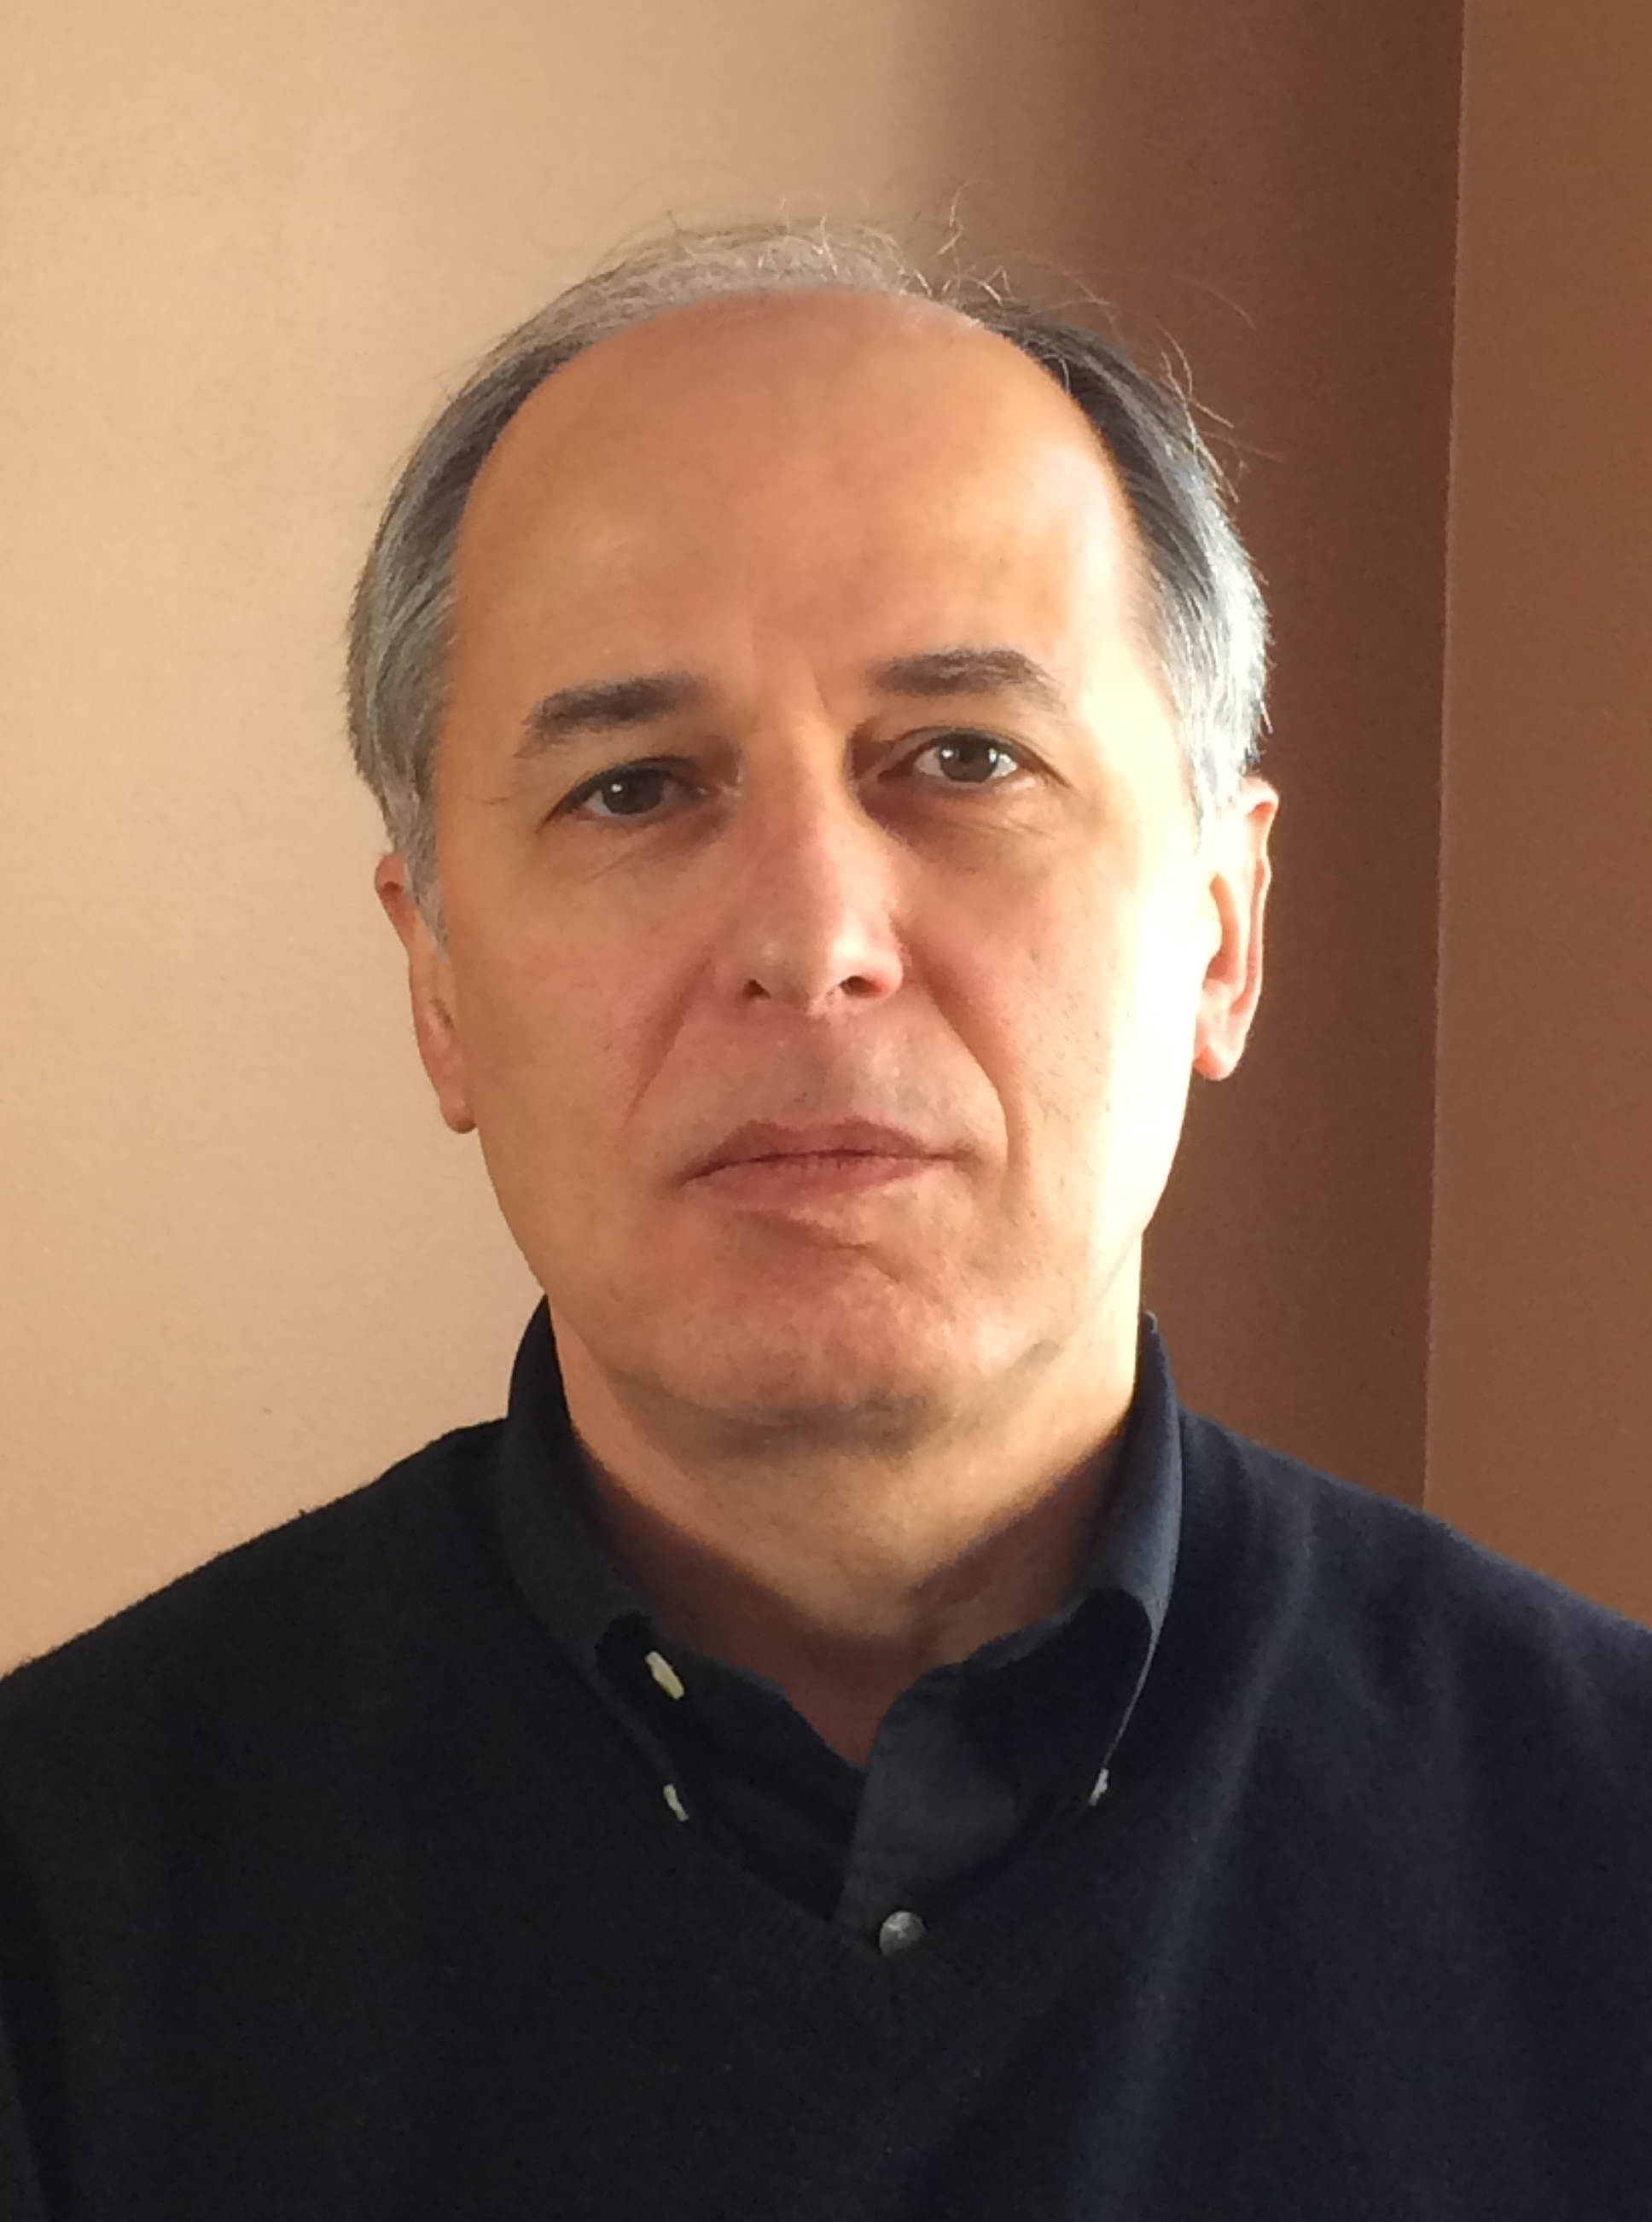
\includegraphics[width=0.35\textwidth]{Images/fominphoto.jpg}
            \hfill
            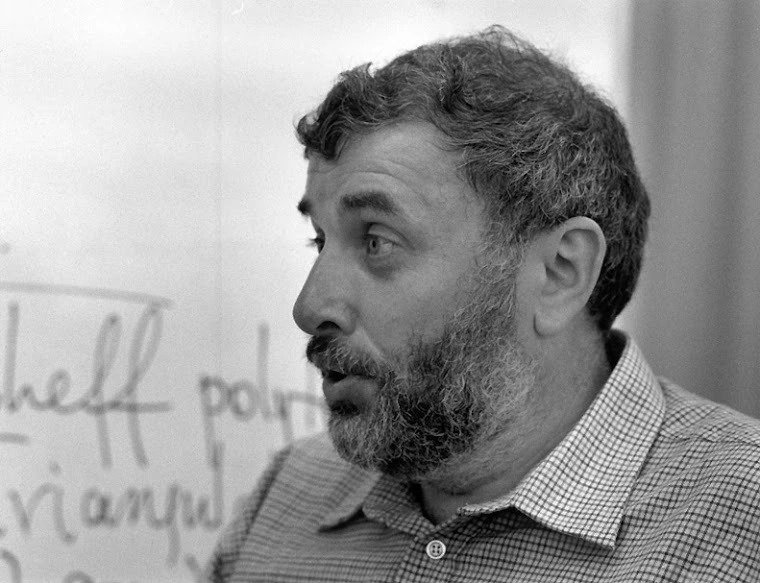
\includegraphics[width=0.4\textwidth]{Images/zelevinskiphoto.jpeg}
        \caption{Cluster algebra was first introduced, in 2002, by Sergey Fomin and Andrei Zelevinsky.}
        \label{fig:my_label}
    \end{figure}
\end{frame}

\begin{frame}{Introduction}
    Where are Cluster algebras encountered?
    \pause
    \begin{itemize}
        \item Frieze patterns,
        \item Triangulated surfaces,
        \item Coxeter groups,
        \item Number theory,
        \item Hyperbolic geometry,
        \item Combinatorics,
        \item Quiver representations...
    \end{itemize}
\end{frame}

\begin{frame}{Introduction}
    Where are Cluster algebras encountered?
    \begin{itemize}
        \item Frieze patterns,
        \item \textcolor{red}{Triangulated surfaces},
        \item Coxeter groups,
        \item \textcolor{red}{Number theory},
        \item \textcolor{red}{Hyperbolic geometry},
        \item \textcolor{red}{Combinatorics},
        \item Quiver representations...
    \end{itemize}
\end{frame}

\begin{frame}{Cluster algebras}
    $(\mathcal{G}, \cdot)$ a free abelian group with basis $\{y_1,\dots,y_n\}$.
    \pause
    Define $\oplus$ by 
    \begin{equation*}
        \prod y_j^{a_j}\oplus\prod y_j^{b_j} = \prod y_j^{\min(a_j,b_j)};
    \end{equation*}
    \pause
    e.g. $y_1^3y_2^{-4}y_3\oplus y_1^{-1}$ $= y_1^{-1}y_2^{-4}$.
\end{frame}
    
\begin{frame}{Cluster algebras}
    Consider $(\mathcal{G}, \oplus, \cdot)$; \pause  then take its group ring $\mathbb{Z}\mathcal{G}$ (also known as a \emph{tropical semifield}). This will be our ambient field\footnote{$\mathbb{Z}\mathcal{G}$ is exactly the ring of Laurent polynomials.}.
\end{frame}

%\begin{frame}{Cluster algebras}
%    A \emph{Cluster algebra} $\mathcal{A} = \mathcal{A}(\mathbf{x},\mathbf{y},\mathcal{Q})$, 
 %   where,
%    \pause
%    \begin{itemize}
%        \item $\mathbf{x}$ is an $n$-tuple of variables, called the initial \emph{Cluster};
 %       \pause
 %       \item $\mathbf{y}$ is the basis of our free abelian group; called the initial \emph{coefficients};
 %       \pause
 %       \item $\mathcal{Q}$ is a \emph{cluster Quiver}.
    
 %   \end{itemize}
%\end{frame}

\begin{frame}{Cluster algebras}
     A \emph{seed} $(\mathbf{x},\mathbf{y},\mathcal{Q})$ determines the corresponding Cluster algebra $\mathcal{A} = \mathcal{A}(\mathbf{x},\mathbf{y},\mathcal{Q})$ through a few rules; where
     \pause
    \begin{itemize}
        \item $\mathbf{x}=(x_1,\dots,x_n)$ is the   $n$-tuple of variables, called the \emph{initial cluster}; e.g. in the setting of triangulated polygons, these are precisely the diagonals of the triangulation.
        \pause
        \item $\mathbf{y}=(y_1,\dots,y_n)$ is the $n$-tuple of generators, called the \emph{initial coefficients}; e.g. in the setting of Conway-Coxeter Frieze patterns, all these variables are equal to 1. 
        \pause
        \item $\mathcal{Q}$ a cluster quiver.
    \end{itemize}
\end{frame}

\begin{frame}{Cluster algebras}
    A \emph{quiver} $\mathcal{Q}$ is a directed graph; i.e. a $4$-tuple $(\mathcal{Q}_0, \mathcal{Q}_1, h, t)$.
    \begin{itemize}
        \item $\mathcal{Q}_0$ is the set of vertices $\{1,2,\dots, n\}$; \pause
        \item $\mathcal{Q}_1$ is the set of arrows,\pause
        \item $h,t : \mathcal{Q}_0 \to \mathcal{Q}_1$, where $h$ maps the head of the arrow and $t$ maps the tail, each to the appropriate vertex.
    \end{itemize}
    \pause
\begin{figure}[H]
    \centering
    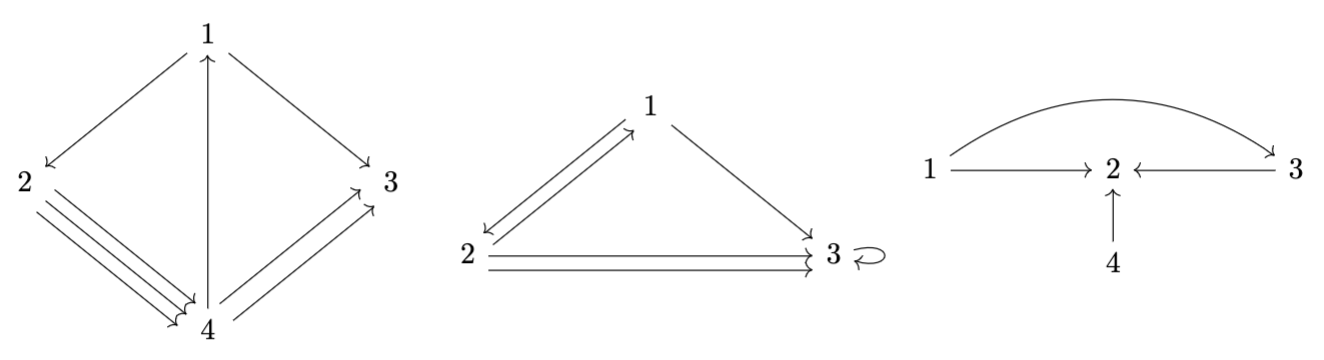
\includegraphics[width = 11 cm]{Images/quivers.png}
    \caption{Example of 2 \emph{cluster quivers} (left and rightmost) and a non-cluster quiver (middle)}
    \label{fig:my_label}
\end{figure}
\end{frame}

\begin{frame}{Cluster algebras}
The Cluster algebra is generated by applying a recursive method to the initial seed, called a \emph{cluster mutation}. A \emph{cluster mutation} $\mu_k$ acts on $\bold{x}$ as follows; $\mu_k((x_1,\dots,x_k,\dots, x_n)) = (x_1,\dots,x'_k,\dots,x_n)$, where; \pause
\begin{equation*}
    x'_k = \dfrac{1}{y_k \oplus 1}\dfrac{y_k\prod_{i \to k}x_i + \prod_{k \to j}x_j}{x_k}.
\end{equation*}
\end{frame}

\begin{frame}{Cluster algebras}
A mutation $\mu_k$ also yields a new quiver $\mathcal{Q}'$ in the following way: \pause
\begin{itemize}
    \item [1.] For any path $i \to k \to j$ add an arrow $i \to j$;\pause
    \item[2.] Invert all arrows going into, or coming out from, vertex $k$; \pause
    \item[3.] Cancel any 2-cycle.
\end{itemize}
\pause
    \begin{figure}[H]
        \centering
        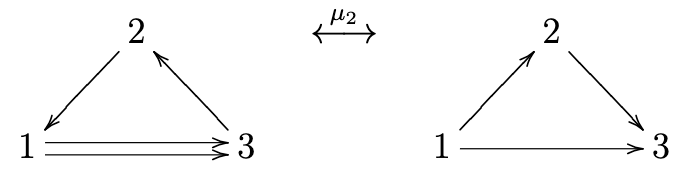
\includegraphics[width = 10 cm]{Images/mutationexample.png}
        \caption{Example of mutation.}
        \label{fig:my_label}
    \end{figure}
\end{frame}
\section{Frobenius' Conjecture}
\begin{frame}{Frobenius' Conjecture}
    Markov's equation:
    \begin{equation*}
        x^2 + y^2 + z^2 = 3xyz;
    \end{equation*}
    \\
\pause
e.g. $(1, 5, 13), (5, 13, 194), (1, 89, 233), (5, 29, 433)$.
\end{frame}

\begin{frame}{Frobenius' Conjecture}
\begin{block}{Conjecture}
Given any two ordered\footnote{An \emph{ordered} Markov triple is a solution $(a,b,c)$ to Markov's equation, such that $a \leq b \leq c$.} Markov triples $(a_1,b_1,c_1)$ and  $(a_2,b_2,c_2)$, if $c_1 = c_2$, then $a_1=a_2$ and $b_1 = b_2$.
\end{block}
\end{frame}

\section{Connection to Cluster algebras}

\begin{frame}{Connection?}
\centering
    How does Cluster algebra factor in when thinking about Frobenius' conjecture?
\end{frame}

\begin{frame}{Connection?}
    Consider the triangulated punctured torus $\mathbb{T}^2$, as the quotient space
    \begin{equation*}
        \mathbb{T}^2 = I \times I/\sim_{vert}/\sim_{hor}, 
    \end{equation*}
    where $I = [0,1] \subset \mathbb{R}$ and $\sim_{vert}$ and $\sim_{hor}$ is the equivalence relation $(x,1)\sim_{vert}(x,0))$, and $(0,y)\sim_{hor}(1,y)$...
    \pause
    \begin{figure}
        \centering
        \includegraphics[width = 5 cm]{figures/Torus.tex}
    \end{figure}
\end{frame}

\begin{frame}{Connection?}
\begin{figure}
    \centering
\includegraphics{figures/TriangTorusMPOrient.tex}
\end{figure}    
\end{frame}

\begin{frame}{Connection?}
\begin{figure}
    \centering
    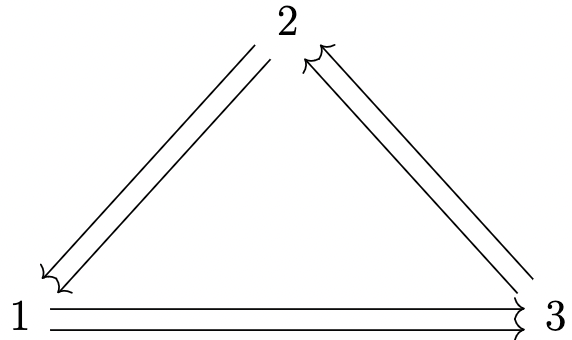
\includegraphics[width = 5 cm
]{Images/MarkovQuiverImgPres.png}
\end{figure}
\end{frame}
\begin{frame}{Connection?}
    Applying a mutation at any vertex, say 1, yields the following Cluster variables; \pause
    \begin{align*}
        (x_1,x_2,x_3) \mapsto &((x_2^2 + x^2_3)/x_1, x_2,x_3) \\
        =&(3x_2x_3 - x_1,x_2,x_3).
    \end{align*} \pause
    \begin{alertblock}{Recall}
        A \emph{cluster mutation} $\mu_k$ acts on $\bold{x}$ as follows; $\mu_k((x_1,\dots,x_k,\dots, x_n)) = (x_1,\dots,x'_k,\dots,x_n)$, where; \pause
\begin{equation*}
    x'_k = \dfrac{1}{y_k \oplus 1}\dfrac{y_k\prod_{i \to k}x_i + \prod_{k \to j}x_j}{x_k}.
\end{equation*}
    \end{alertblock}
\end{frame}

\begin{frame}{Connection?}
\setbeamercovered{transparent}
    Observe that by starting with $(x_1,x_2,x_3) = (1,1,1)$ (the smallest Markov triple), we obtain \pause
    \begin{align*}
    \mu_1(1,1,1) &= (2,1,1) \sim (1,1,2), \\ \pause
    \mu_1(1,1,2) &= (5,1,2) \sim (1,2,5), \\ \pause
    \mu_1(1,2,5) &= (29,2,5) \sim (2,5,29), \\ \pause
    \mu_1(2,5,29) &= (433,5,29) \sim (5,29,433), \\
    & \ \vdots
\end{align*}
\end{frame}

\begin{frame}{Markov Tree}
\begin{figure}
    \centering
    \includegraphics[width = 10 cm]{figures/MarkovNumberTree.tex}
\end{figure}    
\end{frame}

\section{Continued fractions}

\begin{frame}{Continued Fractions}
A continued fraction is a way to represent a real number; as follows, \pausa
\begin{equation*}
    [a_1,a_2,\dots,a_n] = a_1 + \dfrac{1}{a_2+\dfrac{1}{\ddots + \dfrac{1}{a_n}}}.
\end{equation*}
\pause
\begin{exampleblock}{Example}
    Consider the real numbers $22/7,\sqrt{2}$;\pause  then, $22/7 = 3+1/7 = [3;7]$, and 
    \pause
\begin{align*}
    \sqrt{2} &= 1 + \dfrac{1}{2+ \dfrac{1}{2 + \ddots}} = [1;2,2,2,\dots].
\end{align*} 
\end{exampleblock}
\end{frame}


\begin{frame}{Continued Fractions}
    A continued fraction $[a_1,\dots,a_n]$ is called \emph{palindromic of even length} if $(a_1,\dots,a_n) = (a_n,\dots,a_1)$, as sequences and $n$ is even. 
\end{frame}

\section{Snake graphs}

\begin{frame}{Snake graphs}
    A snake graph is a graph that consists of \emph{tiles}; where a tile is \pause
\begin{figure}[H]
    \centering
    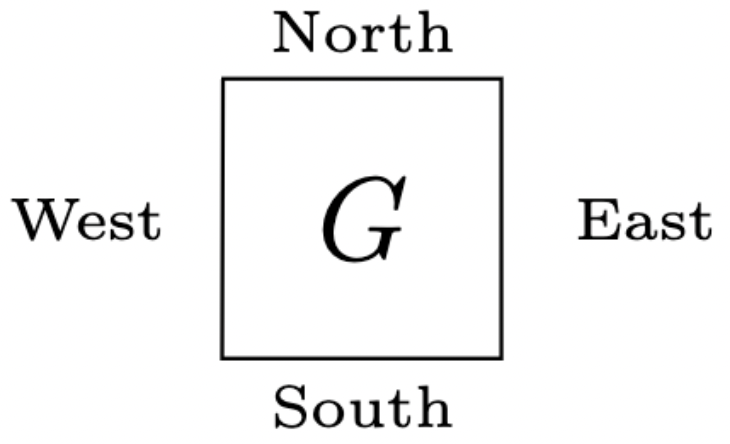
\includegraphics[width = 2.5 cm]{Images/prestile.png}   
\caption{A tile $G$ with sides labeled to denote the orientation}
\pause Any tile can be attached on either the north or east edge of the previous tile.
\end{figure}
\end{frame}

\begin{frame}{Snake graphs}
    Furthermore, on a snake graph, we assign a \emph{sign function}
    \begin{equation*}
    f: \{\text{edges of} \  \mathcal{S}\} \to \{\bplus,\rmin \}.
\end{equation*}
such that for each tile $G_i$ the following hold; \pause
\begin{itemize}
    \item The north and west edge have the same sign, \pause
    \item The south and east edge have the same sign, \pause
    \item The sign on the south edge is different than the sign on the north edge.
\end{itemize}
\end{frame}

\begin{frame}{Snake graphs}
\begin{exampleblock}{Example}
\centering
    \begin{tikzpicture}
        \directlua{tikzsnake("eneennene",4)}
    \end{tikzpicture}
\end{exampleblock}
\end{frame}

\begin{frame}{Snake graph of a continued fraction}
For a continued fraction $[a_1,\dots,a_n]$, we denote by $\mathcal{S}[a_1,\dots,a_n]$ its corresponding snake graph. 
\pause Consider $[a_1,\dots,a_n]$, and the sign sequence 
\begin{equation}\label{signsequence}
\begin{array}{cccccccc}
 %(f(e_0),f(e_1),\ldots,f(e_d)) &=&
  ( \underbrace{ \rmin,\ldots,\rmin},&  \underbrace{ \bplus ,\dots, \bplus},&  \underbrace{ \rmin,\ldots,\rmin},& \ldots,&  \underbrace{\epsilon,\ldots,\epsilon}) ,  \\
 a_1 & a_2 & a_3&\ldots&a_n
\end{array} 
\end{equation}
where $\epsilon = $
$
\begin{cases}
\bplus  \ \text{if} \ n \ \text{is even}; \\
\rmin \ \text{if} \ n \ \text{is odd}
\end{cases}.
$
\end{frame}

\begin{frame}{Snake graph of a continued fraction}
\centering
    Then the snake graph $\s[a_1,\dots,a_n]$ is the graph with precisely $a_1 + \dots + a_n - 1$ tiles determined by its sign sequence.
\end{frame}
\begin{frame}{Snake graph of a continued fraction}
    \begin{exampleblock}{Example}
Consider the fraction $31/7$, with its corresponding continued fraction \pause $[4,2,3]$. We get the sign sequence \pause
$
\begin{array}{ccc}
  ( \rmin,\rmin,\rmin,\rmin,&  \bplus,\bplus,&  \rmin,\rmin,\rmin);
\end{array}
$
which yields the following snake graph;
\pause
\begin{figure}[H]
    \centering
    \begin{tikzpicture}
        \directlua{tikzsnake("eneenne",4)}
    \end{tikzpicture}
\end{figure}
\end{exampleblock}
\end{frame}

\begin{frame}{Snake graph of a continued fraction}
    \begin{theorem}
        If $m(\s)$ denotes the number of perfect matchings of $\s$, then \pause
        \begin{equation*}
            [a_1,a_2,\dots,a_n] = \dfrac{m(\s[a_1,a_2,\dots,a_n])}{m(\s[a_2,a_3,\dots,a_n])}
        \end{equation*}
    \end{theorem}
\end{frame}

\begin{frame}{Snake graph of a continued fraction}

    \begin{exampleblock}{Example}
        If we take $[4,2,3]$, we have \pause
        \begin{align*}
            [4,2,3] &= \dfrac{m\left(\vcenter{\hbox{\begin{tikzpicture}[scale=0.3, transform shape] 
            \directlua{tikzsnake("eneenne",5)}
            \end{tikzpicture}}}
            \right)}{m\left(
            \vcenter{\hbox{\begin{tikzpicture}[scale=0.3, transform shape]
                \directlua{tikzsnake("een",5)}
            \end{tikzpicture}}}
            \right)}\\ 
            &= \dfrac{31}{7}
        \end{align*}
    \end{exampleblock}
\end{frame}

\section{Palindromification}

\begin{frame}{Palindromification}
    Given a continued fraction $[a_1,\dots,a_n]$, we define the continued fraction $[a_n,\dots,a_1,a_1,\dots,a_n]$ to be its \emph{palindromification}. It has the following properties; \pause
    \begin{itemize}
        \item The snake graph $\s[a_n,\dots,a_1,a_1,\dots,a_n]$ has a rotational symmetry at its center tile; \pause e.g. \begin{tikzpicture}[scale=0.3, transform shape]
                \directlua{tikzsnake("enne",5)}. 
            \end{tikzpicture} \pause
        \item If $[a_1,\dots,a_n] = p_n/q_n$, then \pause
        \begin{equation*}
            [a_n,\dots,a_1,a_1,\dots,a_n] = \dfrac{p_n^2 + q_n^2}{p_np_{n-1} + q_nq_{n-1}}; 
        \end{equation*} \pause
        e.g. for $[3,1,5] = 23/6$, we have that $[3,1] = 4$; and $[5,1,3,3,1,5] = \dfrac{565}{98} = \dfrac{23^2 + 6^2}{4\cdot23 + 1 \cdot 6}$.
    \end{itemize}
\end{frame}

\section{Markov numbers \& reformulation of the conjecture}

\begin{frame}{Markov numbers}
By using what we described so far, we can prove the following results; \pause
\begin{itemize}
    \item Every Markov number is the numerator of a palindromic continued fraction of even length that consists only of $1$'s and $2$'s. \pause
    \item Every Markov number (except 1 and 2) is the sum of two relatively prime squares.
\end{itemize}
\end{frame}
\begin{frame}{Reformulations of the conjecture}
    Via the above, we can show that the following conjecture implies Frobenius'; \pause
    \begin{block}{Conjecture}
        Let $m > 2$ be a Markov number. Then there exist \textbf{unique} positive integers $a < b$ with gcd$(a,b) = 1$, such that $m = a^2 + b^2$, $2a \leq b < 3a$; and the continued fraction corresponding to $b/a$ consists entirely of 1's and 2's.
    \end{block}
\end{frame}

\begin{frame}{The End}
    Thank you for listening!

\end{frame}
\end{document}